\section{实验评价}
\label{sec:eval}
\label{sec:experiments}

我们在注入缺陷、模型构建图、收据文本和合同字段上测试修复。共享提示用于测试上下文，过滤前后的评分用于测试门控，人工评审检查参考差异和实际编辑。本文提出三个问题：\textbf{RQ1}：修复何时能改善图？\textbf{RQ2}：上下文、过滤和编辑选择各改变了什么？\textbf{RQ3}：已有图何时比重新抽取更有用？表~\ref{tab:research_answers}~汇总结果。

\subsection{测试设置}
\label{sec:eval:setup}

\paragraph{来源记录与注入缺陷。}
来源数据包含陕西省人民政府的 4,728 条政务记录、国家金融监督管理总局的 1,000 条金融记录，以及生态环境部的 500 条环境记录。我们从每个来源最多抽取 500 篇文档，为每篇构建字段图。

源文本以“字段名：值”列出非空字段，用中文句号连接。每个值最多 320 个字符，服务标签最多 100 个字符。相同的清理后取值构成参考三元组。我们用随机种子 42，按 70/15/15 将文档划分为训练、验证和测试集。在加入缺陷前按来源编号划分，同一原始文档及其修改副本属于同一组。

每张测试图恰好加入两个缺陷。六种缺陷为三元组缺失、三元组重复、非法关系、反向边、无来源支持的值和层级冲突。保存的数据列出每条干净和修改后的三元组。测试集有 225 篇文档，每个来源 75 篇，共 450 个缺陷（表~\ref{tab:repair_benchmark}）。

\begin{table}[t]
\centering
\caption{注入缺陷测试数据。最后三列为文档数。}
\label{tab:repair_benchmark}
\small
\begin{tabular}{l r r r r r}
\toprule
领域 & 文档数 & 缺陷数 & 训练 & 验证 & 测试 \\
\midrule
政务 & 499 & 998 & 349 & 75 & 75 \\
金融 & 500 & 1,000 & 350 & 75 & 75 \\
环境 & 500 & 1,000 & 350 & 75 & 75 \\
\midrule
总计 & 1,499 & 2,998 & 1,049 & 225 & 225 \\
\bottomrule
\end{tabular}
\end{table}

\paragraph{模型构建的图。}
Claude Haiku 为相同的 225 篇测试文档分别构建新图。输入为源文本、文档编号和允许关系。评分器将结构化字段作为参考值。十个响应的 JSON 无效，按空图计分，解析成功率为 95.56\%。共有 77 张图与参考不同，包含 302 项三元组差异。两名评审检查其中固定抽样的 200 项差异，第三名评审解决分歧（第~\ref{sec:eval:human}~节）。

\paragraph{修复方法。}
所有方法获得相同输入图、源文本、文档编号和允许关系。
\begin{itemize}
    \item \textbf{来源字段复制}：读取字段标签，直接从文本复制值。
    \item \textbf{不修复}：返回输入。
    \item \textbf{仅规则}：去重，将指向文档节点的边反向，删除非法头节点和关系。
    \item \textbf{SHACL 风格修复}：使用 SHACL 形状约束检查文档头节点和允许关系\citep{ref_shacl2017}。
    \item \textbf{直接调用模型}：调用一次模型，根据原文返回完整图。
    \item \textbf{ReAct 风格智能体}：一次调用查找错误，另一次调用执行修复\citep{ref_yao2023react}。
    \item \textbf{简单流程}：清理输入，调用一次模型，并对响应去重。
    \item \textbf{诊断＋门控}：在提示中增加错误报告，按文档编号、关系、来源匹配、重复数量和每字段值数量过滤输出。
\end{itemize}

除另行指定模型外，模型方法均在同一端点使用 \texttt{claude-haiku-4-5-20251001}\citep{ref_anthropic_claude45}，温度为零。所有分数均包含失败调用。注入缺陷测试中，直接调用模型 和 简单流程 各有一个无效 JSON 响应，诊断＋门控 和 ReAct 均为零。

\paragraph{评分与统计检验。}
当输出恢复各条干净三元组的数量，并去掉其修改形式时，该缺陷视为修复。我们还衡量正确事实保留、过度修复、三元组 F1、整图精确匹配、调用次数和请求时间。整图精确匹配同时检查三元组与重复数量。

令 $G_0$ 为模型构建的输入图，$G_1$ 为修复图，$G^*$ 为参考图。令 $d$ 统计多余和缺失的三元组，包括重复副本。参考差异减少率为
\[
    1-\frac{d(G_1,G^*)}{d(G_0,G^*)},
\]
该指标在 77 个与参考不同的输入上取平均。负值表示输出差异变多。事实保留和过度修复也按参考三元组计算。人工分数衡量评审是否发现错误、是否接受编辑。

置信区间（CI）使用 10,000 次配对 bootstrap 抽样。匹配测试每次抽取完整文档，使同一文档的两个注入缺陷保持在一起。配对符号随机化检验使用 10,000 次抽样和种子 42。较早的缺陷与整图匹配比较使用精确 McNemar 检验。模型输出差异数还使用单侧配对 Wilcoxon 检验。

首次匹配上下文测试使用未校正的 $p$ 值。后续组件、收据上下文和保存响应测试按各表所列分组进行 Holm 校正。每个 95\% 置信区间对应一个比较，Holm 校正作用于同一检验组的 $p$ 值。

\subsection{注入缺陷修复}
\label{sec:eval:overall}

诊断＋门控 修复 98.00\% 的缺陷，保留 99.32\% 的干净事实，F1 达 99.17\%（表~\ref{tab:repair_main}）。简单流程 使用相同的一次调用上限，修复率为 95.11\%，F1 为 96.34\%。诊断＋门控 修复了 简单流程 漏掉的 15 个缺陷；简单流程 修复了 诊断＋门控 漏掉的两个缺陷（McNemar $p=0.00235$）。配对修复率增益为 2.89 个百分点（95\% 置信区间：1.11--4.89；$p=0.0067$），F1 增益为 2.84 个百分点（95\% 置信区间：1.65--4.25）。直接调用模型 的修复率为 92.44\%。来源字段复制 直接读取记录中的字段名和值，不调用模型，修复率和整图匹配均为 100\%。

\begin{table*}[t]
\centering
\caption{225 篇测试文档、450 个注入缺陷上的修复结果。过度修复、调用数和请求时间越低越好。}
\label{tab:repair_main}
\small
\resizebox{\textwidth}{!}{%
\begin{tabular}{l c c c c c c c}
\toprule
方法 & 缺陷修复 & 事实保留 & 过度修复 & 三元组 F1 & 整图匹配 & 调用／篇 & 耗时／篇 \\
\midrule
来源字段复制 & \textbf{1.0000} & \textbf{1.0000} & \textbf{0.0000} & \textbf{1.0000} & \textbf{1.0000} & 0.00 & $<0.001$ s \\
不修复 & 0.0000 & \textbf{1.0000} & \textbf{0.0000} & 0.7615 & 0.0000 & 0.00 & $<0.001$ s \\
仅规则 & 0.3200 & \textbf{1.0000} & \textbf{0.0000} & 0.8472 & 0.0622 & 0.00 & $<0.001$ s \\
SHACL 风格修复 & 0.0000 & \textbf{1.0000} & \textbf{0.0000} & 0.7998 & 0.0000 & 0.00 & $<0.001$ s \\
直接调用模型 & 0.9244 & 0.9687 & 0.0758 & 0.9520 & 0.8267 & 1.00 & 7.25 s \\
ReAct 风格智能体 & 0.8911 & 0.9324 & 0.1667 & 0.9213 & 0.5956 & 2.00 & 20.50 s \\
简单流程 & 0.9511 & 0.9723 & 0.0705 & 0.9634 & 0.8400 & 1.00 & 9.27 s \\
诊断＋门控 & 0.9800 & 0.9932 & 0.0167 & 0.9917 & 0.9333 & 1.00 & 11.44 s \\
\bottomrule
\end{tabular}%
}
\end{table*}

诊断＋门控 修复了 直接调用模型 漏掉的 28 个缺陷；直接调用模型 修复了 诊断＋门控 漏掉的三个缺陷（$p=4.65\times10^{-6}$）。与 ReAct 比较时，两项计数分别为 42 和二（$p=1.13\times10^{-10}$）。这些检验比较完整修复方法，第~\ref{sec:eval:mechanisms}~节再测试其中步骤。

\begin{figure*}[t]
\centering
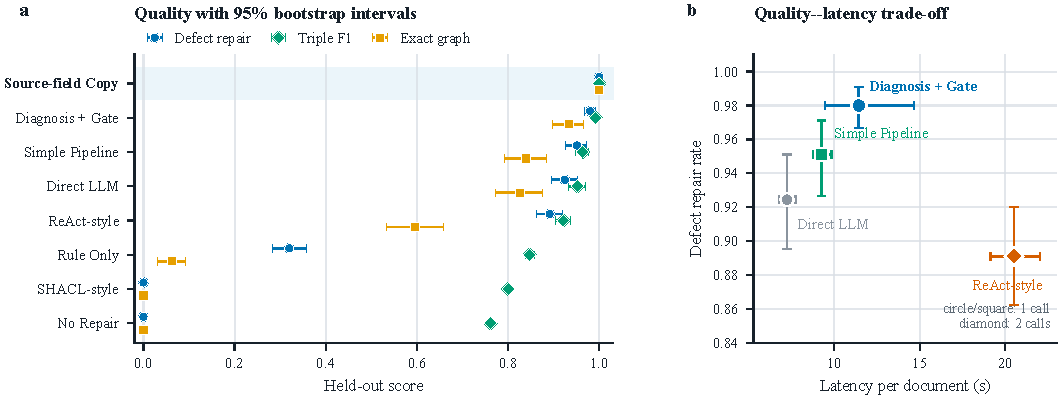
\includegraphics[width=0.98\textwidth]{figure/experiments/repair_benchmark_results.pdf}
\caption{注入缺陷修复。\textbf{a}：修复率、三元组 F1 和整图匹配，带基于文档抽样的 95\% 置信区间。\textbf{b}：一次或两次调用方法的分数与请求时间。}
\label{fig:repair_benchmark_results}
\end{figure*}

\subsection{模型构建图的修复}
\label{sec:eval:natural}

输入图的 F1 为 87.99\%，整图匹配为 65.78\%（表~\ref{tab:natural_errors}）。诊断＋门控 将 F1 提高到 92.48\%，参考差异减少 27.75\%，并保留全部原本匹配参考的输入三元组。简单流程 在 77 个有差异输入上的平均差异减少率为 $-59.15\%$，增加的差异多于去掉的差异。

诊断＋门控 的 F1 比 简单流程 高 4.40 个百分点（95\% 置信区间：3.07--5.77），平均每篇少 1.03 项差异（95\% 置信区间：0.77--1.32；Wilcoxon $p=3.18\times10^{-12}$）。三个图在 诊断＋门控 下完全匹配参考，在 简单流程 下不匹配；反向情况为零（$p=0.25$）。来源字段复制 匹配全部参考。

\begin{table*}[t]
\centering
\caption{模型构建图的修复。差异减少率使用 77 个与参考不同的输入，其余分数使用全部 225 篇文档。}
\label{tab:natural_errors}
\small
\resizebox{\textwidth}{!}{%
\begin{tabular}{l c c c c c c c}
\toprule
方法 & 解析率 & 非精确输入 & 差异减少率 & 事实保留 & 过度修复 & 三元组 F1 & 整图匹配 \\
\midrule
来源字段复制 & 1.0000 & 77 & 1.0000 & 1.0000 & 0.0000 & 1.0000 & 1.0000 \\
抽取图，不修复 & 0.9556 & 77 & 0.0000 & 1.0000 & 0.0000 & 0.8799 & 0.6578 \\
简单流程 & 1.0000 & 77 & $-0.5915$ & 0.9971 & 0.2389 & 0.8807 & 0.6711 \\
诊断＋门控 & 0.9956 & 77 & 0.2775 & 1.0000 & 0.0292 & 0.9248 & 0.6844 \\
\bottomrule
\end{tabular}%
}
\end{table*}

\paragraph{有效与无效 JSON 输入。}
215 个有效 JSON 输入的 F1 为 92.09\%。诊断＋门控 达到 93.53\%，简单流程 为 88.85\%。67 个有效但有参考差异的输入中，诊断＋门控 使差异减少 24.00\%，F1 从 74.61\% 提高到 79.22\%。148 个原本精确匹配的图全部保持精确匹配。十个无效输入修复后的 F1 为 69.91\%，没有一个整图精确匹配。

\begin{figure}[t]
\centering
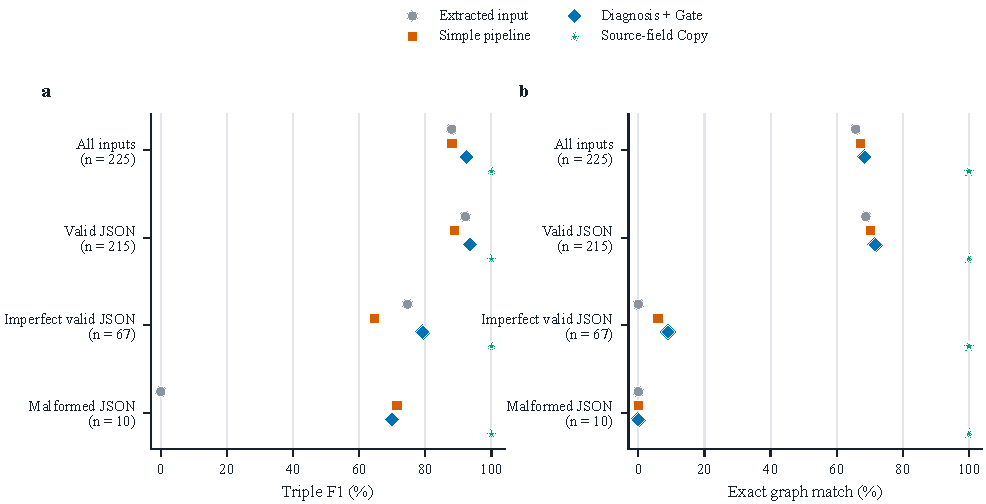
\includegraphics[width=0.98\textwidth]{figure/experiments/natural_stratified.pdf}
\caption{按输入类型划分的修复分数。有效 JSON 组展示可解析图的修复，无效 JSON 组展示空输入的恢复。}
\label{fig:natural_stratified}
\end{figure}

\subsection{提示、过滤与编辑选择器测试}
\label{sec:eval:router}
\label{sec:eval:mechanisms}

我们依次测试提示文本、过滤和编辑选择。在保存的 Claude 响应上，过滤将 F1 从 98.95\% 提高到 99.17\%，过度修复降低 0.60 个百分点。修复率保持 98.00\%，整图匹配保持 93.33\%。过滤器去掉八条三元组，均未通过来源检查且与参考不同。附录~\ref{sec:eval:ablation}~给出完整方法表。

% Begin merged sections/audit_primary.tex
% Generated by exps/paper1_mechanism_audit/write_paper_tables.py
\begin{table*}[t]
\centering
\caption{Gemma 提示测试，每组输入 60 篇文档。每个原始／过滤对照使用同一响应。}
\label{tab:matched_mechanisms}
\small
\resizebox{\textwidth}{!}{%
\begin{tabular}{llrrrr}
\toprule
上下文 & 输出 & 受控修复 & 受控 F1 & 模型构建 F1 & 模型构建整图匹配 \\
\midrule
基础提示 & 未过滤 & 0.9750 & 0.9951 & 0.9185 & 0.6667 \\
基础提示 & 门控 & 0.9750 & 0.9962 & 0.9252 & 0.6667 \\
诊断提示 & 未过滤 & 0.9250 & 0.9850 & 0.9079 & 0.6667 \\
诊断提示 & 门控 & 0.9250 & 0.9861 & 0.9147 & 0.6667 \\
SHACL 上下文 & 未过滤 & 0.9500 & 0.9912 & 0.9322 & 0.7000 \\
SHACL 上下文 & 门控 & 0.9500 & 0.9912 & 0.9364 & 0.7000 \\
\bottomrule
\end{tabular}%
}
\end{table*}
% End merged sections/audit_primary.tex


Gemma 测试使用 60 篇文档，每个来源 20 篇，分别测试注入缺陷输入和模型构建输入。三个提示共享指令、清理步骤、温度和输出上限。每个响应在同一门控过滤前后计分。表~\ref{tab:matched_mechanisms}~给出六种设置，表~\ref{tab:matched_cost}~给出输入 token 数和请求时间。第~\ref{sec:impl:shacl}~节给出 SHACL 提示。

经过过滤，基础提示在注入缺陷输入上达到 99.62\% F1 和 97.50\% 修复率。错误报告提示为 98.61\% F1 和 92.50\% 修复率。配对 F1 变化为 $-1.01$ 个百分点（95\% 置信区间：$[-1.67,-0.38]$；$p=0.0082$）。模型构建输入上，基础提示 + 门控 的 F1 为 92.52\%，诊断＋门控 为 91.47\%，SHACL 上下文＋门控 为 93.64\%。诊断 与 SHACL 的 F1 差为 $-2.16$ 个百分点（95\% 置信区间：$[-5.26,0.02]$；$p=0.105$）。

在使用错误报告提示的模型构建输入上，过滤将 F1 从 90.79\% 提高到 91.47\%，增益为 0.69 个百分点（95\% 置信区间：0.20--1.29；$p=0.0335$），整图匹配保持相同。360 个响应共拒绝 27 条三元组，均与参考不同。

\begin{figure}[t]
\centering
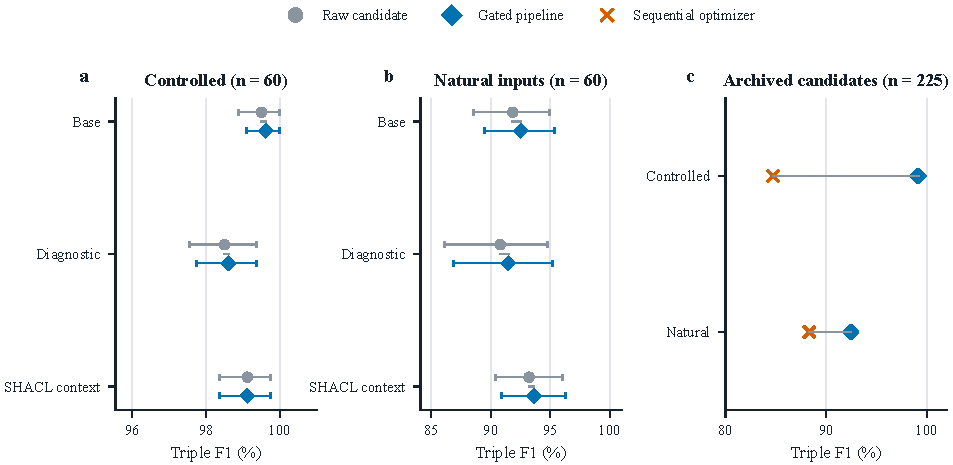
\includegraphics[width=0.98\textwidth]{figure/experiments/matched_mechanisms.pdf}
\caption{提示、过滤和选择器测试。a--b 使用 60 篇文档的 Gemma 输出；每个原始／过滤对照使用同一响应，误差线表示 95\% 文档 bootstrap 置信区间。c 使用 225 篇文档保存的 Claude 建议。}
\label{fig:matched_mechanisms}
\end{figure}

% Begin merged sections/factorial_controls.tex
\paragraph{联合测试清理、错误报告与过滤。}
\label{sec:eval:factorial}

我们分别开启或关闭输入清理（$P$）与错误报告（$D$）。四种提示设置使用 60 个注入缺陷输入和 60 个模型构建输入，得到 480 个 Gemma 响应。每个响应分别在启用和关闭门控（$G$）时计分。每项主效应都对另外两个开关取平均。

\begin{table}[t]

\centering

\caption{平均 F1 变化，单位为百分点。每组输入有 60 篇配对文档，各效应对另外两个开关取平均。区间为 95\% 文档 bootstrap 置信区间。$p_H$ 对六项主效应检验进行 Holm 校正。}
\label{tab:recovery_factorial}

\small

\begin{tabular}{llrrr}

\toprule

输入 & 组件 & 变化 & 95\% 区间 & $p_H$ \\

\midrule

受控输入 & 预处理 & -0.028 & [-0.797, 0.778] & 1.000 \\

受控输入 & 诊断 & -0.651 & [-1.348, -0.056] & 0.164 \\

受控输入 & 门控 & +0.164 & [0.054, 0.301] & 0.156 \\

模型构建输入 & 预处理 & +0.697 & [0.000, 1.905] & 1.000 \\

模型构建输入 & 诊断 & -0.535 & [-2.376, 0.842] & 1.000 \\

模型构建输入 & 门控 & +0.707 & [0.225, 1.316] & 0.086 \\

\bottomrule

\end{tabular}

\end{table}

六项 Holm 校正后的 $p$ 值均大于 0.05（表~\ref{tab:recovery_factorial}）。错误报告在两组输入中都降低平均 F1。门控在注入缺陷输入上提高 0.164 个百分点，在模型构建输入上提高 0.707 个百分点。所有输入组共拒绝 47 条三元组，其中 17 条文档编号错误，30 条未通过来源匹配，均与参考不同。公开分数还列出开关联合效应和每项检查去掉的候选。


\paragraph{各项过滤检查。}
我们将 540 个已保存响应经过八种过滤设置，得到 4,320 个输出。完整过滤器拒绝 28 条三元组，其中 11 条文档编号错误，17 条来源匹配失败，均与参考不同。其他检查在该样本中未额外去掉候选。21 项检查比较的校正后 $p$ 值均大于 0.05。附录~\ref{sec:eval:individual_ablation}~给出结果表。

\paragraph{编辑选择。}
在保存的 Claude 建议上，默认选择器无论使用学习权重还是等权重，在注入缺陷输入上都接受零项编辑。修复率保持 32.00\%，F1 保持 84.72\%，与清理后输入相同。v2 运行中，模型构建输入的等权重 F1 为 88.33\%，学习权重为 87.99\%，学习触发器也为 87.99\%。去掉编辑成本将注入缺陷 F1 提高到 89.30\%，该设置的模型构建 F1 为 88.13\%。日志显示，一些评估分数较高的图仍缺少字段。某些有用的添加得到不大于零的分数，因而被拒绝。附录~\ref{sec:eval:individual_ablation}~给出全部 13 种设置、两种先验评分形式和 11,700 个结果。附录~\ref{app:historical_diagnostics}~还给出早期选择器结果和调用策略测试。

\subsection{两个模型的测试}
\label{sec:eval:crossmodel}

我们在 60 个注入缺陷输入上比较 直接调用模型、简单流程 和 诊断＋门控，每个来源 20 个。模型为 Claude Haiku 和 \texttt{google/gemma-4-26B-A4B-it}\citep{ref_gemma4}。每种方法跨模型使用相同输入、提示形式、温度和一次调用上限。诊断＋门控 在两个模型上的修复率均最高（表~\ref{tab:cross_model}）。它相对 简单流程 的 F1 优势在 Claude 上更大。Gemma 直接输出的 F1 高于 Claude。

\begin{table}[t]
\centering
\caption{两个模型在相同 60 个注入缺陷输入上的结果。}
\label{tab:cross_model}
\small
\begin{tabular}{l l c c c}
\toprule
模型 & 方法 & 修复率 & F1 & 精确匹配 \\
\midrule
Claude & 直接 & 0.958 & 0.970 & 0.867 \\
Claude & 简单流程 & 0.958 & 0.966 & 0.833 \\
Claude & \textbf{诊断＋门控} & \textbf{0.975} & \textbf{0.991} & \textbf{0.917} \\
\midrule
Gemma & 直接 & 0.958 & 0.988 & 0.883 \\
Gemma & 简单流程 & 0.967 & 0.984 & 0.867 \\
Gemma & \textbf{诊断＋门控} & \textbf{0.983} & \textbf{0.990} & \textbf{0.917} \\
\bottomrule
\end{tabular}
\end{table}

% Begin merged sections/receipt_followup.tex
\subsection{新收据上的来源行提示}
\label{sec:eval:receipt_followup}

首次 60 张收据测试中，基础提示和错误报告提示都保留全部输入图不变。过滤将 F1 从 79.44\% 降到 79.15\%。一个地址因空白与来源不同而被拒绝。49 项参考差异中，有 27 项涉及大小写、空白、标点或金额格式（附录~\ref{sec:eval:external_receipts}）。据此，我们加入字段含义、来源行提示和共享空白规则。

我们用 20 张新收据设置索引设计，然后固定设计，在另外 60 张收据上测试（第~\ref{sec:framework:field_evidence}~节）。首次 60 张、开发 20 张和新测试 60 张收据的编号不同，空白清理后的文本也不同。抽样种子为 20260923。所有预测保存后才下载测试标签。每种方法得到相同字段含义、带行号原文、输入图和指令。简单流程 直接使用这些输入；证据索引 增加字段行提示；SHACL 增加规则检查上下文。三种方法的过滤器使用相同空白规则。

开发集 F1 为：输入 80.00\%，简单流程 82.50\%，证据索引 85.00\%，SHACL 80.00\%。测试保留一个索引设计和全部三种方法。主要比较为 证据索引 减 简单流程 的文档平均 F1。代码和评分规则在测试前固定。

\begin{table*}[t]
\centering
\caption{60 张新收据的修复。各方法共享字段含义、来源行和空白检查。精确匹配使用有标签字段。}
\label{tab:receipt_followup}
\small
\begin{tabular}{lrrrr}
\toprule
方法 & 三元组 F1 & 整图匹配 & 规范化 F1 & 事实保留 \\
\midrule
抽取输入 & 0.7833 & 0.3500 & 0.7958 & 1.0000 \\
简单流程, 未过滤 & 0.7875 & 0.2833 & 0.8083 & 0.9250 \\
简单流程, 过滤后 & 0.7875 & 0.2833 & 0.8083 & 0.9250 \\
证据索引, 未过滤 & 0.8333 & 0.4000 & 0.8625 & 0.9306 \\
证据索引, 过滤后 & 0.8351 & 0.4000 & 0.8643 & 0.9306 \\
SHACL 上下文，未过滤 & 0.7833 & 0.2833 & 0.8042 & 0.9347 \\
SHACL 上下文，过滤后 & 0.7833 & 0.2833 & 0.8042 & 0.9347 \\
\bottomrule
\end{tabular}
\end{table*}

新测试集的输入 F1 为 78.33\%。过滤后 简单流程、证据索引、SHACL 分别为 78.75\%、83.51\%、78.33\%。简单流程 比输入高 $0.42$ 个百分点（95\% 置信区间：$[-4.17,5.00]$）。证据索引 比 简单流程 高 $4.76$ 个百分点（95\% 置信区间：$[2.50,7.26]$；配对随机化 $p=0.0004$）。三种方法的整图匹配分别为 28.33\%、40.00\%、28.33\%。

输入有 52 个字段与参考不同。简单流程 恢复其中 16 个，并丢失 15 个原本精确匹配的字段。证据索引 恢复 26 个、丢失 14 个；SHACL 恢复 13 个、丢失 13 个。索引修正了 11 项标点差异和 6 项文本边界差异。它丢失的 14 个精确匹配中，有 10 个数值金额相同，只改变显示格式。

金额检查去掉总额字段中的货币前缀和千位分隔符。正确金额数为：输入 58/60，简单流程 59/60，证据索引 59/60，SHACL 58/60。清理大小写和空白后，证据索引 的 F1 为 86.43\%，简单流程 为 80.83\%。索引同时提高精确和清理后文本分数。

过滤器拒绝 1 个候选。它与参考不同，并将地址片段拼成原文中没有的文本。被拒绝的参考匹配候选数为 0。过滤使索引 F1 提高 0.18 个百分点，另外两种方法的 F1 保持不变。

简单流程、证据索引、SHACL 分别修改 31、39、28 个输入图。平均修复请求时间为 7.91、7.88、8.11 秒，平均输入长度为 1784、2153、3404 个 token。240 次请求产生 60 个抽取输出和 180 个修复输出。请求时间包含间隔等待和重试。每个原始与过滤后评分对只使用一个响应。

\begin{figure}[t]
\centering
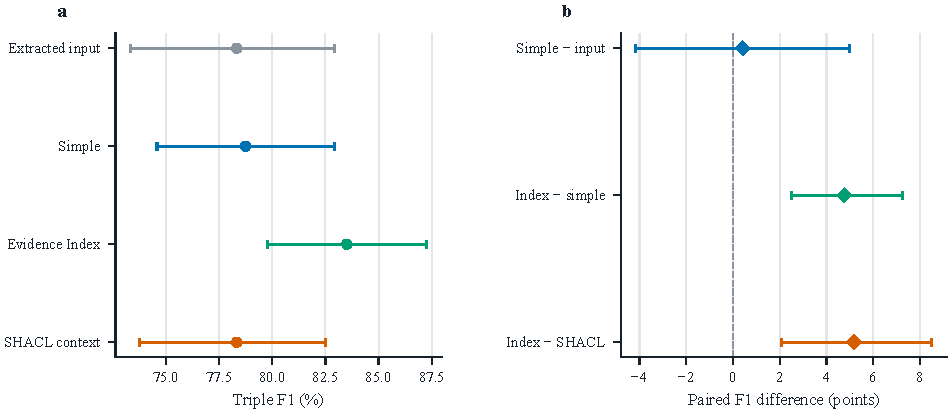
\includegraphics[width=0.98\textwidth]{figure/experiments/receipt_followup.pdf}
\caption{新收据测试。左：平均 F1 及 95\% 文档 bootstrap 置信区间。右：配对 F1 变化。所有方法共享字段含义和来源行。}
\label{fig:receipt_followup}
\end{figure}
% End merged sections/receipt_followup.tex

% Begin merged sections/receipt_context_controls.tex
\subsection{来源行提示对照}
\label{sec:eval:recovery_ablation}

我们在相同 60 张新测试收据上比较六种提示设置。测试使用与组件测试同批的 360 个新 Gemma 响应，全部解析成功。各设置都保留完整原文，并共享模型、输出上限和过滤器。随机索引的字符长度与完整索引大致相同。

\begin{table}[t]

\centering

\caption{60 张收据上的来源行测试。各行使用相同模型、原文、输出上限和过滤器。随机提示与索引的字符长度大致相同。}
\label{tab:recovery_index}

\small

\begin{tabular}{lrr}

\toprule

上下文 & 精确 F1 & 规范化 F1 \\

\midrule

简单流程 & 0.7917 & 0.8125 \\

完整索引 & 0.8351 & 0.8643 \\

仅锚点 & 0.8351 & 0.8643 \\

随机索引 & 0.8167 & 0.8458 \\

简单流程，无字段定义 & 0.8083 & 0.8292 \\

完整索引，无字段定义 & 0.7470 & 0.7762 \\

\bottomrule

\end{tabular}

\end{table}

完整索引的 F1 比 简单流程 高 4.35 个百分点（95\% 置信区间：1.25 至 7.86）。五项预设比较的 Holm 校正值为 $p_H=0.065$。完整索引与仅锚点行的平均 F1 相同。完整索引与随机索引相差 1.85 个百分点（置信区间：$[-0.65,4.52]$；$p_H=0.696$）。去掉字段含义使完整索引 F1 下降 8.81 个百分点（置信区间：$[4.23,13.39]$；$p_H=0.006$）。本批次 简单流程 去掉字段含义后得分更高。这些结果说明字段含义有助于索引提示选择取值。

\begin{figure}[t]

\centering

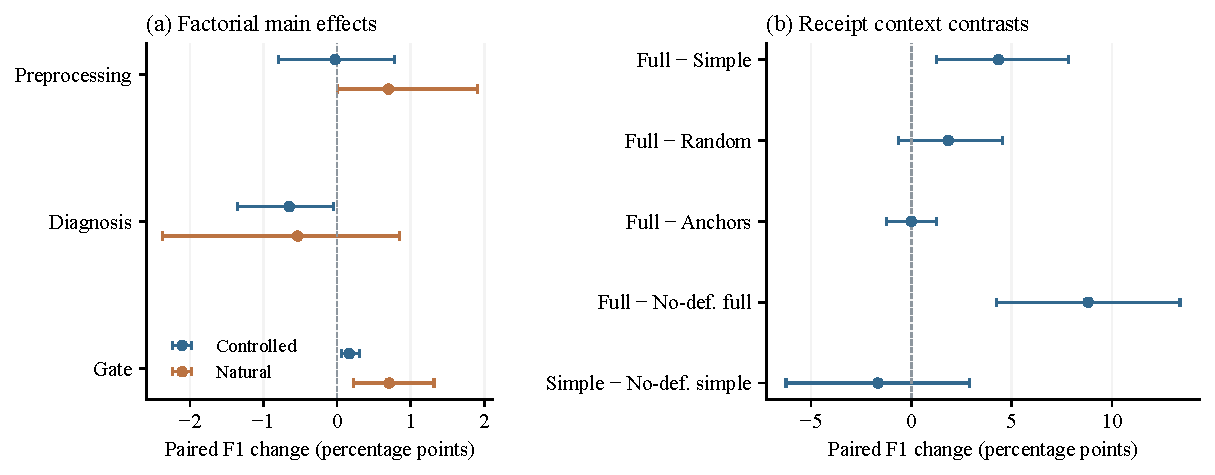
\includegraphics[width=0.98\textwidth]{figure/experiments/recovery_ablation.pdf}

\caption{组件与来源行测试。点表示平均配对 F1 变化，误差线为各项变化的 95\% 置信区间。组件测试与收据测试分别进行 Holm 校正。}
\label{fig:recovery_ablation}

\end{figure}
% End merged sections/receipt_context_controls.tex

% Begin merged sections/reextraction_recovery.tex
\subsection{修复与重新抽取}
\label{sec:eval:reextraction}

我们复用 60 张新测试收据，比较有无索引下的修复与重新抽取，共四种设置。各设置共享来源行、字段含义、文档编号和输出上限；修复额外获得已有图。全部 240 个响应都将 JSON 放在 Markdown 代码围栏中，固定的严格解析器将其计为失败。

随后，我们去掉代码围栏，并为每个输出指定已知文档编号，对相同响应重新计分。这项补充分析得到索引修复 F1 为 83.93\%，索引重新抽取为 74.86\%，配对差为 9.07 个百分点（95\% 置信区间：5.22 至 13.10）。修复调用使用已有图，其构建成本另计。附录~\ref{app:reextraction_diagnostics}~给出严格评分、围栏清理评分、编号错误和来源行覆盖。合同测试在采集前固定围栏处理和编号分配。

% Begin merged sections/cuad_contracts.tex
\subsection{合同字段测试}
\label{sec:eval:cuad}

我们用 CUAD\citep{ref_cuad} 测试五个字段：文档名称、签约日期、生效日期、到期日期或初始期限，以及适用法律。选择空白清理后每字段最多一个不同参考值、原文不超过 40,000 字符的合同。保留完整原文，并检查标注值的位置。20 份官方训练合同构成开发集；全部 56 份满足规则的官方测试合同构成测试集。

比较初始抽取、简单流程 修复、索引修复和索引重新抽取。两种修复方法得到相同初始图，索引方法在完整原文之外增加字段行窗口。各设置共享 Gemma 模型、字段含义和 4,000 token 输出上限。采集前，程序已设置 JSON 围栏处理和文档编号分配。一轮开发之后，提示与选择规则保持固定。

\begin{table}[t]
\centering
\caption{56 份文档的合同结果。F1 检查空白清理后的精确文本。“丢失”统计被删除的正确输入事实。输入行给出初始图成本，修复行给出修复调用成本。}
\label{tab:cuad}
\small
\begin{tabular}{lrrrr}
\toprule
输出 & F1 (\%) & 丢失 & 新增不匹配 & 请求数 \\
\midrule
初始抽取 & 46.76 & 0 & 0 & 59 \\
简单流程修复 & 43.35 & 7 & 2 & 71 \\
索引修复 & 44.84 & 5 & 12 & 69 \\
索引重新抽取 & 44.12 & 8 & 32 & 71 \\
\bottomrule
\end{tabular}
\end{table}

索引修复 F1 为 44.84\%，输入为 46.76\%，下降 1.92 个百分点。它删除五条正确输入事实，并增加十二条与参考不同的事实。简单流程 修复也低于输入。

索引修复的 F1 比索引重新抽取高 0.72 个百分点（95\% 配对置信区间：[-4.80,6.48]；符号翻转检验 $p=0.810$）。测试共用 270 次请求得到 224 个输出，包括重试。失败输出计为空图。评分在空白清理后，将复制文本与 CUAD 标签比较。

\begin{figure}[t]
\centering
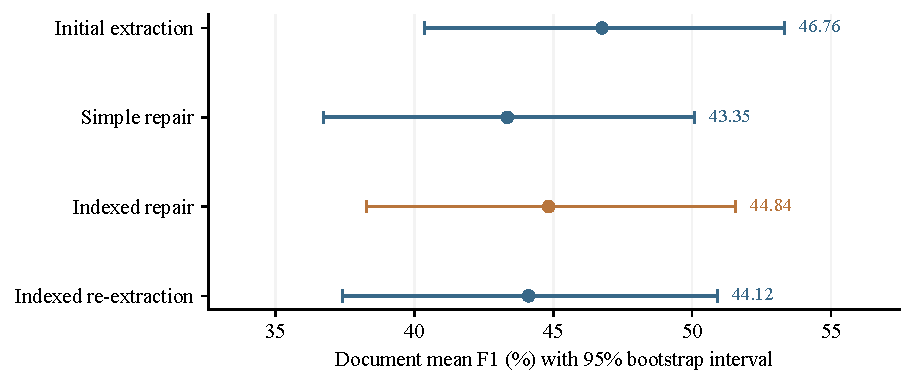
\includegraphics[width=0.88\textwidth]{figure/experiments/cuad_contracts.pdf}
\caption{合同分数。点表示文档平均 F1，误差线为各方法的 95\% 置信区间。正文给出修复与抽取的配对差值区间。}
\label{fig:cuad}
\end{figure}
% End merged sections/cuad_contracts.tex


\subsection{错误与编辑的人工评价}
\label{sec:eval:human}

任务 D 从模型构建输入的 302 项三元组差异中抽取 200 项参考差异。任务 E 从五种设置的 598 项编辑中抽取 200 项实际编辑。两者都用种子 42 随机抽样。每项是一项差异或编辑，同一文档可提供多项。评审看到原文、模式、输入图和指定操作。任务 E 还展示完整输出图。方法名称与参考质量提示隐藏。

两名具有计算机背景和中文阅读能力的评审先阅读规则和练习样例，再各自独立标注相同的 400 项。每项回答两个问题：输入在该位置是否有错（\texttt{is\_error}），以及添加或删除操作是否可接受（\texttt{repair\_acceptable}）。标签为 0、1 或 U，并说明理由。U 表示所示证据不足以作出判断。第三名评审检查原文和图，在两人的答案中选择，解决 154 项分歧。其余 246 项保留一致标签。一项编辑接受判断仍为 U。原始标签和一致性分数均保留。

\begin{table}[t]
\centering
\caption{人工评分。一致率和 $\kappa$ 使用两位评审原始的 0/1/U 答案。正例数使用最终标签，接受率使用答案为 0 或 1 的项目。}
\label{tab:human_review}
\small
\begin{tabular}{llrrrr}
\toprule
任务 & 判断 & 一致率 & $\kappa$ & 正例／确定项 & U \\
\midrule
D & 输入错误 & 80.0\% & 0.600 & 95/200 (47.5\%) & 0 \\
D & 建议编辑可接受 & 62.0\% & 0.334 & 86/200 (43.0\%) & 0 \\
E & 输入错误 & 86.0\% & 0.677 & 134/200 (67.0\%) & 0 \\
E & 实际编辑可接受 & 65.0\% & 0.128 & 134/199 (67.3\%) & 1 \\
\bottomrule
\end{tabular}
\end{table}

评审在 95/200 项参考差异中发现输入错误，接受 86/200 项建议编辑，以及 134/199 项实际编辑，另有一项不确定。一个缺失值本身可以是正确的，但添加后可能使仅允许一个值的字段出现两个值。输入错误与编辑接受问题分别覆盖这两个判断。任务 E 的原始编辑一致率为 65.0\%，$\kappa=0.128$。

\begin{table}[t]
\centering
\caption{按设置划分的实际编辑接受率。随机样本的各组大小不同，比例使用有明确判断的编辑。}
\label{tab:human_review_by_config}
\small
\begin{tabular}{lrrr}
\toprule
配置 & 抽样数 & 可接受 & U \\
\midrule
历史简单流程 & 105 & 63/104 (60.6\%) & 1 \\
历史诊断＋门控 & 41 & 25/41 (61.0\%) & 0 \\
Gemma 基础提示＋门控 & 16 & 13/16 (81.3\%) & 0 \\
Gemma 诊断＋门控 & 16 & 13/16 (81.3\%) & 0 \\
Gemma SHACL 上下文＋门控 & 22 & 20/22 (90.9\%) & 0 \\
\bottomrule
\end{tabular}
\end{table}

样本包含 105 项 历史简单流程 编辑、41 项 历史诊断＋门控 编辑、16 项 Gemma 基础提示＋门控 编辑、16 项 Gemma 诊断＋门控 编辑，以及 22 项 Gemma SHACL 上下文＋门控 编辑。表中按各组报告被接受编辑的比例。

\subsection{讨论}
\label{sec:eval:failure}

来源格式影响修复方法的选择。对于列出字段名和值的记录，解析器可以直接复制字段；收据则需要从全文中选择取值。新收据测试中，来源行提示提高 F1。后续索引测试展示字段含义的作用：去掉后，索引 F1 下降 8.81 个百分点。合同索引修复 F1 为 44.84\%，输入为 46.76\%。保留正确输入字段是清楚的改进目标。

实验还展示过滤器改变了什么。来源和文档编号检查去掉多余三元组。字段选择发生在模型生成和首值规则中。例如，来源可能同时包含小计和最终金额，修复方法必须为“total”选出正确的一个。因此，检查需要同时考虑关系含义和取值是否出现在原文中。

人工评审接受五种设置合并样本中 67.3\% 的编辑，并在 47.5\% 的参考差异样本中发现输入错误。历史诊断＋门控 样本中，接受的编辑为 25/41。结合原始标签和理由，这些分数帮助定位字段选择与单项编辑决策中的错误。

\subsection{代码与数据}

代码、提示、数据名单、模型输出和评分脚本位于 \url{https://github.com/turambar928/MCP_based_KG_construction}。每次运行保存模型设置、解析状态、请求和 token 用量，全部响应均保留。各实验 README 给出数据来源、样本、校验值和运行命令。

人工评价文件包含固定任务规则、评分器、汇总结果、原始一致性分数和样本名单。个人答案与理由不公开。收据评分使用 SROIE 的人工字段标签。

\begin{table}[t]
\centering
\caption{研究问题与测试结果。}
\label{tab:research_answers}
\small
\begin{tabularx}{\textwidth}{@{}p{0.10\textwidth}XX@{}}
\toprule
问题 & 比较 & 结果 \\
\midrule
RQ1 & 注入缺陷与模型构建图
& 诊断＋门控改善修复率和 F1。直接复制匹配全部中文记录参考。 \\
RQ2 & 共享提示与响应；来源行提示；编辑选择器
& 来源和编号检查去掉多余三元组。收据索引提高 F1。匹配测试中，错误报告降低平均 F1。模型构建输入上，等权选择器得分高于学习权重。 \\
RQ3 & 收据、合同修复与重新抽取
& 收据测试在围栏和编号清理后倾向已有图。合同索引修复得分低于初始图。 \\
\bottomrule
\end{tabularx}
\end{table}
